\section{Auswertung}
\label{sec:Auswertung}

\subsection{Bestimmung der Zeitkonstante durch den Entladevorgang}
\label{subsec:Aufgabe_A}
Die Entladungskurve wurde betrachtet.
Die aufgenommenen Messwerte sind in \autoref{tab:data_a} zu finden.
Diese werden in ein halblogarithmischem Diagramm dargestellt, siehe \autoref{fig:data_a}.
Dabei werden die letzten beiden Wertepaare aus \autoref{tab:data_a} nicht mitaufgezeichnet, da der Logarithmus für 0 nicht definiert ist.
Mithilfe von python wird eine lineare Ausgleichsrechnung durchgeführt.
Über die Steigung wird die Zeitkonstante $RC$ ermittelt.
Dafür wurd die Gleichung \eqref{eqn:AufgabeA} betrachtet.

\noindent
Aus der Ausgleichsrechung folgt:
\begin{align*}
  RC &= (1.05 \pm 0.04) \cdot 10^{-3} \si{\second},
  b  &= (6.24 \pm 0.14) \cdot 10^{-3} \si{\second}.
\end{align*}

\begin{table}
  \centering
  \caption{Aufgenommene Messwerte: Die Kondensatorspannung $U_C$ in Abhängigkeit von der Zeit.
  Die letzten beiden Wertepaare wurden nicht in den halblogarithmischem Diagramm aufgenommen.}
  \label{tab:data_a}
  \begin{tabular}{c c}
    \toprule
    $t [\si{\milli\second}]$ & $U_C [\si{\volt}]$ \\
    \midrule
      0     &     6.2  \\
      0.2   &     5.4  \\
      0.4   &     4.0  \\
      0.6   &     3.6  \\
      0.8   &     3.0  \\
      1.0   &     2.0  \\
      1.2   &     2.2  \\
      1.6   &     1.5  \\
      1.8   &     1.0  \\
      2.0   &     0.9  \\
      2.4   &     0.7  \\
      2.8   &     0.5  \\
      3.2   &     0.4  \\
      4.0   &     0.1  \\
    \bottomrule
  \end{tabular}
\end{table}

\begin{figure}
  \centering
  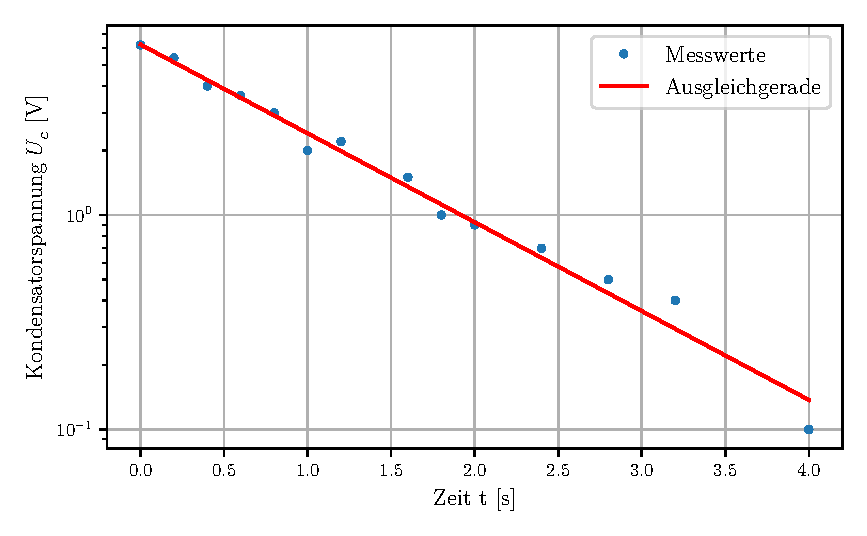
\includegraphics{content/data_a_ausgleich.pdf}
  \caption{Die Kondensatorspannung $U_C$ in Abhängigkeit zur Zeit $t$ und die dazugehörige Ausgleichsgerade.}
  \label{fig:data_a}
\end{figure}

\subsection{Bestimmung der Zeitkonstante durch die Amplitude}
\label{subsec:Aufgabe_B}
Nach dem Anlegen einer Sinusspannung, wird die Amplitude $U_A$ in Abhängigkeit von der Frequenz $f$ aufgenommen.
Die Messpaare sind in \autoref{tab:data_b} zu finden.
Die Werte werden in ein halblogarithmischem Diagramm eingetragen, siehe \autoref{fig:data_b} und eine nicht-lineare Ausgleichsrechnung wird nach Gleichung \eqref{eqn:amplitude} durchgeführt.

\noindent
Aus dieser Rechung ergibt sich für 
\begin{equation*}
  RC = (-5.92 \pm 1.35) \cdot 10^{-3} \si{\second}.
\end{equation*}

\begin{table}
  \centering
  \caption{Aufgenommene Messwerte: Die Kondenssatorspannungsamplitude $U_A$ in Abhängigkeit der Frequenz $f$.}
  \label{tab:data_b}
  \begin{tabular}{c c}
    \toprule
    $f [\si{\hertz}]$ & $U_A [\si{\volt}]$ \\
    \midrule
    10.41       &   3.20    \\
    30.07       &   3.10    \\
    50.00       &   3.00    \\
    100.00      &   2.55    \\
    150.00      &   2.15    \\
    200.10      &   1.80    \\
    300.00      &   1.40    \\
    500.00      &   0.90    \\
    750.00      &   0.65    \\
    1000.00     &   0.50    \\
    1500.00     &   0.34    \\
    2001.00     &   0.26    \\
    3005.00     &   0.17    \\
    5003.00     &   0.105   \\
    7500.00     &   0.072   \\
    10000.00    &   0.054   \\
    \bottomrule
  \end{tabular}
\end{table}

\begin{figure}
  \centering
  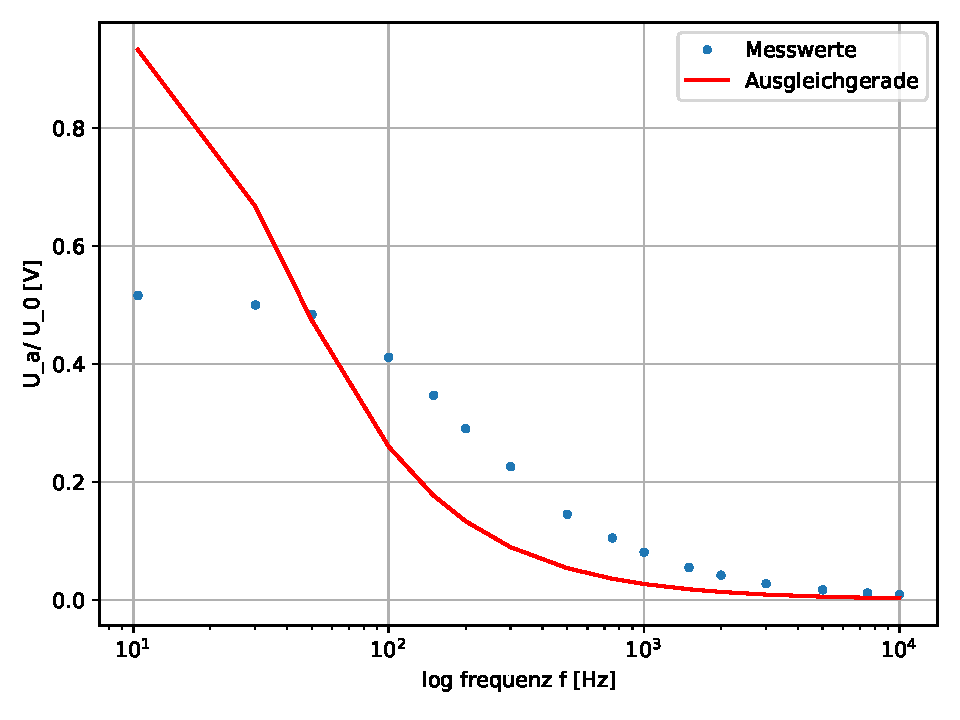
\includegraphics{content/data_b_ausgleich.pdf}
  \caption{Die Kondenssatorspannungsamplitude $U_A$ in Abhängigkeit der Frequenz $f$ und die dazugehörige Ausgleichskurve.}
  \label{fig:data_b}
\end{figure}


\subsection{Bestimmung der Zeitkonstante durch die Phasenverschiebung}
\label{subsec:Aufgabe_C}
Die nach \autoref{} aufgenommenen Messwerte sind in \autoref{tab:data_c} zu finden.
Mithilfe der Gleichung \autoref{} wird die Phasenverschiebung $\phi$ ermittelt, welche auch in \autoref{tab:data_c} zu sehen sind.
Es folgt eine Aufnahme der Phasenverschiebung in Abhängigkeit von der Frequenz $f$ in einem halblogarithmischen Diagramm, siehe \autoref{fig:data_c}.
Durch eine Ausgleichsrechnung nach Gleichung \eqref{eqn:phasenverschiebung} folgt für die Zeitkonstante
\begin{equation*}
  RC = (-0.92 \pm 0.14) \cdot 10^{-3}.
\end{equation*}

\begin{table}
  \centering
  \caption{Aufgenommene Messwerte: Der zeitliche  Abstand $a$ und die Wellenlänge $b$ in Abhängigkeit der Frequenz $f$, sowie die daraus resultierende Phasenverschiebung $\phi$.}
  \label{tab:data_c}
  \begin{tabular}{c c c c}
    \toprule
    $f [\si{\hertz}]$ & $a [\si{\milli\second}]$ & $b [\si{\milli\second}]$ & $\phi$ \\
    \midrule
    10.41       &     1.000     &   98.00   &   \\
    30.07       &     1.000     &   33.00   &   \\
    50.00       &     1.000     &   19.50   &   \\
    100.00      &     0.800     &   10.00   &   \\
    150.00      &     0.800     &    6.80   &   \\
    200.10      &     0.700     &    5.00   &   \\
    300.00      &     0.500     &    3.30   &   \\
    500.00      &     0.400     &    2.00   &   \\
    750.00      &     0.280     &    1.30   &   \\
    1000.00     &     0.200     &    1.00   &   \\
    1500.00     &     0.160     &    0.66   &   \\
    2001.00     &     0.110     &    0.49   &   \\
    3005.00     &     0.100     &    0.32   &   \\
    5003.00     &     0.045     &    0.20   &   \\
    7500.00     &     0.030     &    0.13   &   \\
    10000.00    &     0.030     &    0.10   &   \\
    \bottomrule
  \end{tabular}
\end{table}

\begin{figure}
  \centering
  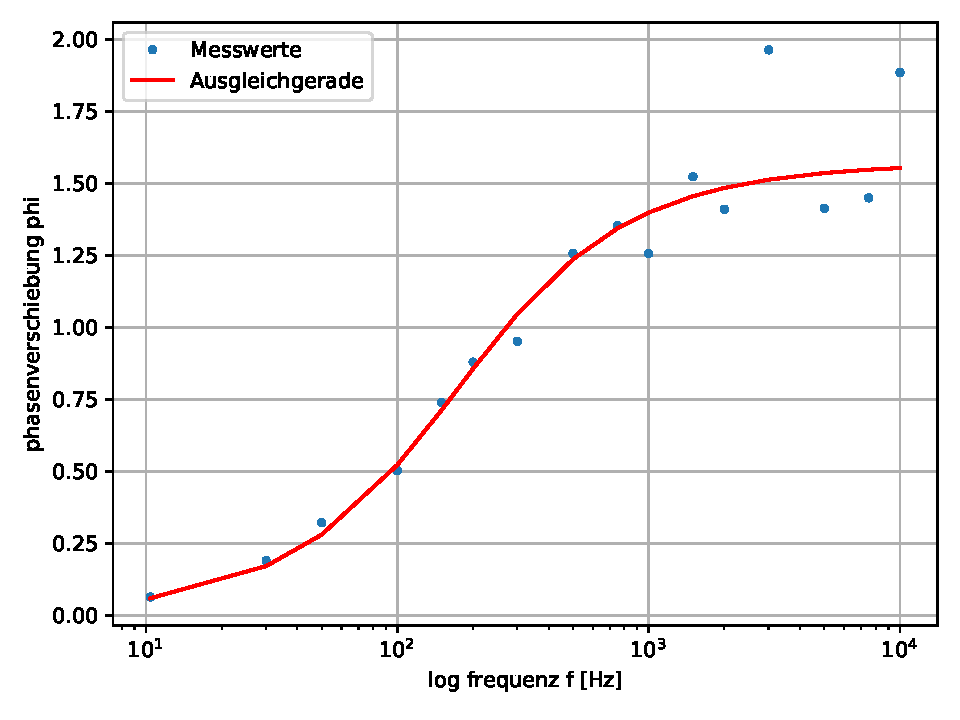
\includegraphics{content/data_c_ausgleich.pdf}
  \caption{Die Phasenverschiebung $\phi$ in Abhängigkeit von der Frequenz $f$ und die dazugehörige Ausgleichskurve.}
  \label{fig:data_c}
\end{figure}

\subsection{RC-Kreis als Integrator}
\label{Aufgabe_d}
Mithilfe der Gleichung \eqref{eqn:AufgabeD} soll die Relativamplitude $\sfrac{A(\omega)}{U_0}$ der Phase $\phi$ in ein Polarkoodinatensystem eingetragen werden.
Dafür wird die Zeitkonstante $RC$ aus \autoref{subsec:Aufgabe_C} verwendet.
In der \autoref{fig:data_d} werden zusätzlich einige Messwerte eingetragen.

\begin{figure}
  \centering
  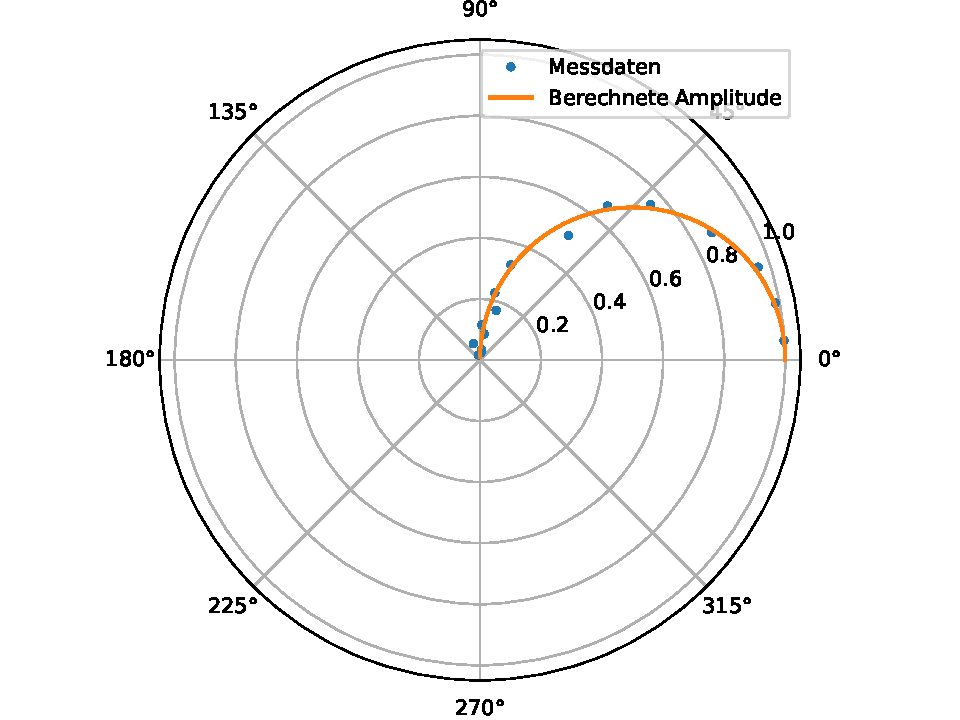
\includegraphics{content/data_d_ausgleich.pdf}
  \caption{Die Relativamplitude, sowie einige Messwerte.}
  \label{fig:data_d}
\end{figure}
%
%-----------------------------------
%AUFGABE A) 
%log U_c = RC*t + b
%
%a = -0.9540848364455892
%b = 1.841404733455546
%a fehler = 0.03658725999310259
%b fehler= 0.07137530467922369
%----------------------------------
%AUFGABE A
%RC = 1.048235250026088
%b = 6.24166772868657
%RC fehler = 0.04090898460866068
%b fehler= 0.13887375836089974
%
%AUFGABE B
%RC = -0.005917848334705116
%RC fehler = 0.0013479645549506188
%
%AUFGABE C
%RC = -0.0009174386895810928
%RC fehler = 0.00013536682656469667
%
%
%